\chapter{Experiments and Headroom}
\index{Experiments and Headroom@\emph{Experiments and Headroom}}

For our experiments we used GPGPUsim with a variety of programs from the Rodinia 2.0 \cite{rodinia} and Lonestar 2.0 \cite{lonestar} benchmark suites. Later in this section, we present promising results for applying Hawkeye to our GPU simulator environment. However, due to the lack of both time and domain knowledge, we were only able to gather basic headroom data for our idea of cache precleaning. In the following sections we will describe the details of the simulator used, discuss properties of our benchmarks and platform such as cache sensitivity and bandwidth usage, and finally present our headroom and actual performance improvements using Hawkeye and precleaning.

\section{Simulator}
We use the GPGPUsim \cite{gpgpusim} simulator for our experiments, targeting the provided configuration that approximates the Nvidia Fermi architecture. This architecture supports 15 cores, each core consisting of 32 SIMD lanes and a maximum of 48 scheduled warps. Each core has a private 16 KB, 4-way set associative L1 cache with 128 bytes lines, and the entire system has a shared 786 KB, 8-way set associative L2 cache with 128 byte lines. The L2 cache is split into 12 portions and assigned to the 12 separate DRAM memory partitions. Finally, the L1 cache acts as write-through cache while the L2 cache acts as a write-back cache.

GPGPUsim runs CPU code natively, then intercepts CUDA library calls in order to perform full functional simulation (as opposed to a trace-based simulation). Because GPGPUsim doesn’t provide an option for trace-based simulation, we cannot skip warmup cycles and our simulations take significant amount of time to run to completion. Due to these restrictions, our simulations were sometimes cut short and compared against a baseline that ran for the same amount of time. Unfortunately this means that our results are often extrapolated and could be inaccurate.

The version of GPGPUsim used is a slight modification of the 3.0 release that has basic support for CUDA 5.5. This modified version is used in order to be able to run the Lonestar 2.0 benchmark suite. Furthermore, we made use of the AerialVision \cite{aerialvision} visualization software provided with GPGPUsim, but we made minor modifications in order to display the precleaning data presented in this report.

The baseline caches used within the simulator are all managed by a standard implementation of LRU (no pseudo timestamps are used). Furthermore, as is common on GPUs, the caches have no prefetching and they only cache global reads/writes (accesses to shared memory are on chip and are thus equivalent to an L1 access). All atomic operations skip the L1 cache, and writes cause evictions from the L1 cache.

\section{Cache Sensitivity}
Cache sensitivity tells us how much cache performance affects a given benchmark. We would expect that a benchmark with heavy code divergence or a small memory footprint would have little to no improvements even from an optimal cache implementation. By enlarging the cache and measuring the change in instructions per clock (IPC) over our baseline, we can get a rough approximation of how much a given benchmark relies on the cache. If we see little to no improvement when enlarging the cache, we wouldn't expect a change in replacement policy to have much affect on performance either. Benchmarks with large IPC improvements have high cache sensitivity and benchmarks that do roughly the same as baseline are considered to have low cache sensitivity. In our Hawkeye experiments, we would like to see large performance improvements on benchmarks that have high cache sensitivity, but see performance on par with LRU in benchmarks with low cache sensitivity. This experiment was motivated by the same study done by the APCM paper as referenced in our Related Work section earlier.

In order to measure L1 cache sensitivity we quadrupled the size of our L1 cache and compared IPC performance against our baseline cache described above. We also repeated this experiment for our L2 cache. Our results for this experiment are presented below in Figure \ref{f:sensitivity} in Appendix A. Interestingly enough, we see that a number of graph algorithms including MST, SSSP, and BFS exhibit high levels of cache sensitivity. Graph algorithms on GPU tend to do poorly due to their irregular and hard to predict access patterns. The other interesting thing to note here is that between two runs of bfs we see different levels of cache sensitivity, this could be due to how the two data sets were generated or the differing sizes of the data sets. Another interesting thing to note is when increase the cache size for some of our benchmarks we actually perform even worse. We believe this strange result can be explained by Belady’s anomaly \cite{belady_anomaly}.


\section{Hawkeye}
For evaluating Hawkeye on GPU we first evaluate both PC and PC combined with warp ID as training features by comparing prediction biases. Next we evaluate real performance impact by measuring the change in IPC over our LRU baseline. Overall, we find that Hawkeye does well compared to LRU, though there is no clear winner between our PC and PC+WID features.

To begin, we measured the per-feature bias of the OPTGen algorithm for both the PC and PC+WID features. Per-feature bias essentially tells us the prediction quality of our chosen feature, it tells us how often our predictions on a feature agree with each other. We note that the two hotspot benchmarks have a 100\% per-feature bias. We believe this high bias is caused by a well optimized code base that provides a small amount of PC values (a max of 4 in our simulations). The full set of per-feature biases for L1 and L2 caches can be seen in Figures \ref{f:l1_bias} and \ref{f:l2_bias} respectively.

\begin{figure}[htb]
\begin{center}
\ 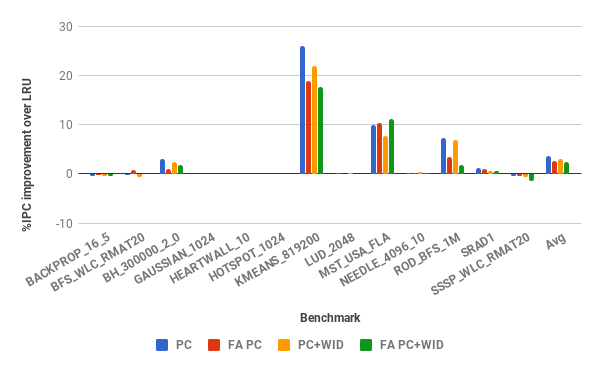
\psfig{file=figs/l1_ipc.png,width=\textwidth}
\caption{IPC improvements over baseline when applying Hawkeye to L1 caches. Improvements are measured with both PC and PC+WID features and also with default (4-way associate) and fully associative OPTgen training. FA denotes the fully-associative OPTgen training.}
\label{f:l1_ipc}
\end{center}
\end{figure}

\begin{figure}[htb]
\begin{center}
\ 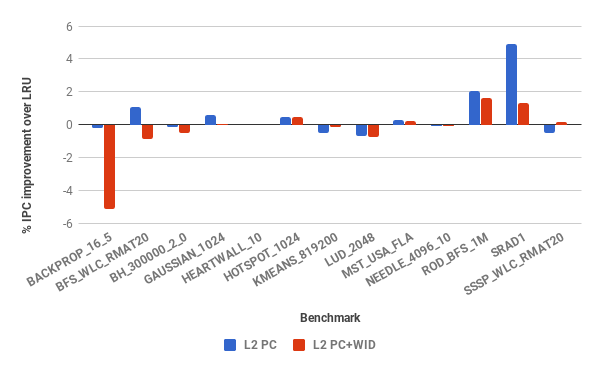
\psfig{file=figs/l2_ipc.png,width=\textwidth}
\caption{IPC improvements over baseline when applying Hawkeye to L2 caches.}
\label{f:l2_ipc}
\end{center}
\end{figure}

An important difference between our PC and PC+WID features that's not displayed in our bias metric is the larger number of values being trained on for PC+WID. In Figure \ref{f:opt_uniq_vals} is a plot of the number of unique values seen per feature. This large increase in potential feature values requires adequate hardware to track, and more values being trained typically leads to slower training times. In Figure \ref{f:cpu_opt_uniq_vals} we present the number of unique PC values seen by OPTGen when running on a last level cache on a CPU using SPEC 2006 \cite{spec} benchmarks and ChampSim \cite{champsim}. The number of unique values seen for PC+WID on GPU and PC on CPU are roughly on the same order of magnitude. We believe there is more room for complex feature experimentation, especially involving dynamic warp IDs or better hashing algorithms.

In our full performance tests we measured two important metrics: post-warmup cache miss rate, and IPC improvement over baseline. For the post-warmup miss rate metric, we ignore all cache misses before a specified warmup time, as most misses at the beginning of a program are compulsory and cannot be avoided. We found that a post-warmup time of 3,000,000 cycles fits most of the benchmarks being used (with the exception of HOTSPOT which ends before 3,000,000 cycles). We present the miss rate improvements over LRU for L1 and L2 caches in Figures \ref{f:l1_miss_rate} and \ref{f:l2_miss_rate}. As mentioned above, PC hashed with warp ID ends up performing better than just PC. We present IPC improvements for L1 and L2 caches in Figures \ref{f:l1_ipc} and \ref{f:l2_ipc}.

The performance gains seen at the L1 level are encouraging, as we see significant performance improvements on a few benchmarks. Hawkeye applied to L2 caches gives less significant results, but this is mostly in line with what we found in our cache sensitivity study above. It appears as though, across the board, PC is currently the best feature to use with Hawkeye on GPUs at both the L1 and L2 level. Furthermore, we believe that training OPTgen on a fully-associative cache isn't a good choice as we consistently see performance drops compared to the default OPTGen.

\section{Precleaning}

The results for our idea of precleaning include a coarse measure of headroom and performance tests of basic predictors we tried. The headroom tests give a basic, yet idealized view of how much room we have to improve. Like our Hawkeye results, we measure performance benefits in IPC improvement over baseline with no precleaning enabled.

For our headroom study we measure performance improvement when assuming no cost for executing a write-back. In a completely ideal scenario, a precleaner would be able to completely hide the effects of write-back being sent to main memory. This experiment also gives us an idea of which benchmarks are bandwidth sensitive, much like our cache sensitivity study earlier. We refer to Figure \ref{f:preclean_headroom} for the results of our headroom. [Elaborate when data comes in.]

We also implemented a basic implementation of what we consider a functional precleaning unit. This precleaning unit was implemented in the L2 cache, using a slight modification to Cache Burst \cite{cache_burst} to predict when a line should be precleaned. Referring to Figure \ref{f:preclean_perf} we see little impact to performance with our implementation of a precleaning unit.

Our idea of precleaning certainly needs more evaluation and exploration of prediction mechanisms beyond what is provided in this report. We believe with more time and better domain knowledge we could make real performance improvements. Though it remains uncertain if these performance improvements would be significant enough to warrant the cost of an entirely new L2 prediction unit that needs to evaluate precleaning candidates, clean lines, and predict bandwidth usage on a regular basis.
